\documentclass{beamer} % Использование класса beamer для создания презентации
\setbeamerfont{framesubtitle}{size=\large}

\usetheme{Boadilla} % Применение темы Boadilla

\usepackage[T2A]{fontenc} % Установка кодировки шрифта
\usepackage[utf8]{inputenc} % Установка кодировки исходного текста
\usepackage[english,russian]{babel} % Подключение локализации и переносов для русского и английского языков
\usepackage{amsmath,amssymb} % Подключение математических символов и формул
\usepackage{autonum} % Автоматическая нумерация формул только при наличии ссылок на них
\usepackage{wrapfig} % Подключение пакета для обтекания текстом рисунков и таблиц
\usepackage{array} % Подключение пакета для работы с таблицами
\usepackage{booktabs}

\newcommand{\PreserveBackslash}[1]{\let\temp=\\#1\let\\=\temp} % Команда для сохранения обратной косой черты в ячейках таблицы
\newcolumntype{C}[1]{>{\PreserveBackslash\centering}p{#1}} % Создание нового типа столбца с центрированным содержимым

\usepackage[labelformat=empty]{caption} % Подключение пакета для настройки подписей и удаление названия "Рисунок"
\graphicspath{{./images/}} % Указание папок, где искать изображения

\setbeamertemplate{navigation symbols}{} % Удаление навигационных символов на слайдах
\usepackage{ragged2e} % Подключение пакета для улучшенного выравнивания текста
\newcommand{\jj}{\righthyphenmin=20 \justifying} % Команда для активации выравнивания по ширине с установкой минимального количества символов в слове перед переносом

\date{\today}

\begin{document}

\begin{frame}
  \begin{center}\tiny
    Федеральное государственное автономное образовательное учреждение высшего образования \\
    «Национальный исследовательский университет ИТМО»\\
    Факультет систем управления и робототехники
  \end{center}

  \begin{center}\tiny
    \textbf{\MakeUppercase{ВЫПУСКНАЯ КВАЛИФИКАЦИОННАЯ РАБОТА БАКАЛАВРА \\ ПО НАПРАВЛЕНИЮ 15.03.06 <<Мехатроника и робототехника>>}}\\
    \vspace{0.2cm}
    \textbf{\MakeUppercase{на тему:}}\\
    \vspace{0.1cm}
    \textbf{\MakeUppercase{<<Исследование и сравнение современных алгоритмов
    компьютерного зрения \\ для отслеживания перемещения объектов на видеоизображениях в
    городской среде>>}}
  \end{center}

  \vspace{0.3cm}

  \begin{columns}
    \begin{column}{0.50\textwidth}
      \begin{center}\small
        Выполнил: \\
        \vspace{0.1cm}
        \textbf{Лалаянц Кирилл Артемович}\\
        студент группы R34352 \\
        336700\\
      \end{center}
    \end{column}

    \begin{column}{0.50\textwidth}
      \begin{center}\small
        Научный руководитель:\\
        \vspace{0.1cm}
        \textbf{Шаветов Сергей Васильевич} \\
        доцент, к.т.н., заместитель декана ФСУиР,
        начальник ДНИР \\
      \end{center}
    \end{column}
  \end{columns}

  \vspace{0.5cm}
  \begin{center}\tiny
    Санкт-Петербург \\
    $2025$
  \end{center}
\end{frame}

\begin{frame}
  \frametitle{Информация для предзащиты}
  \framesubtitle{Антиплагиат}
  \centering
  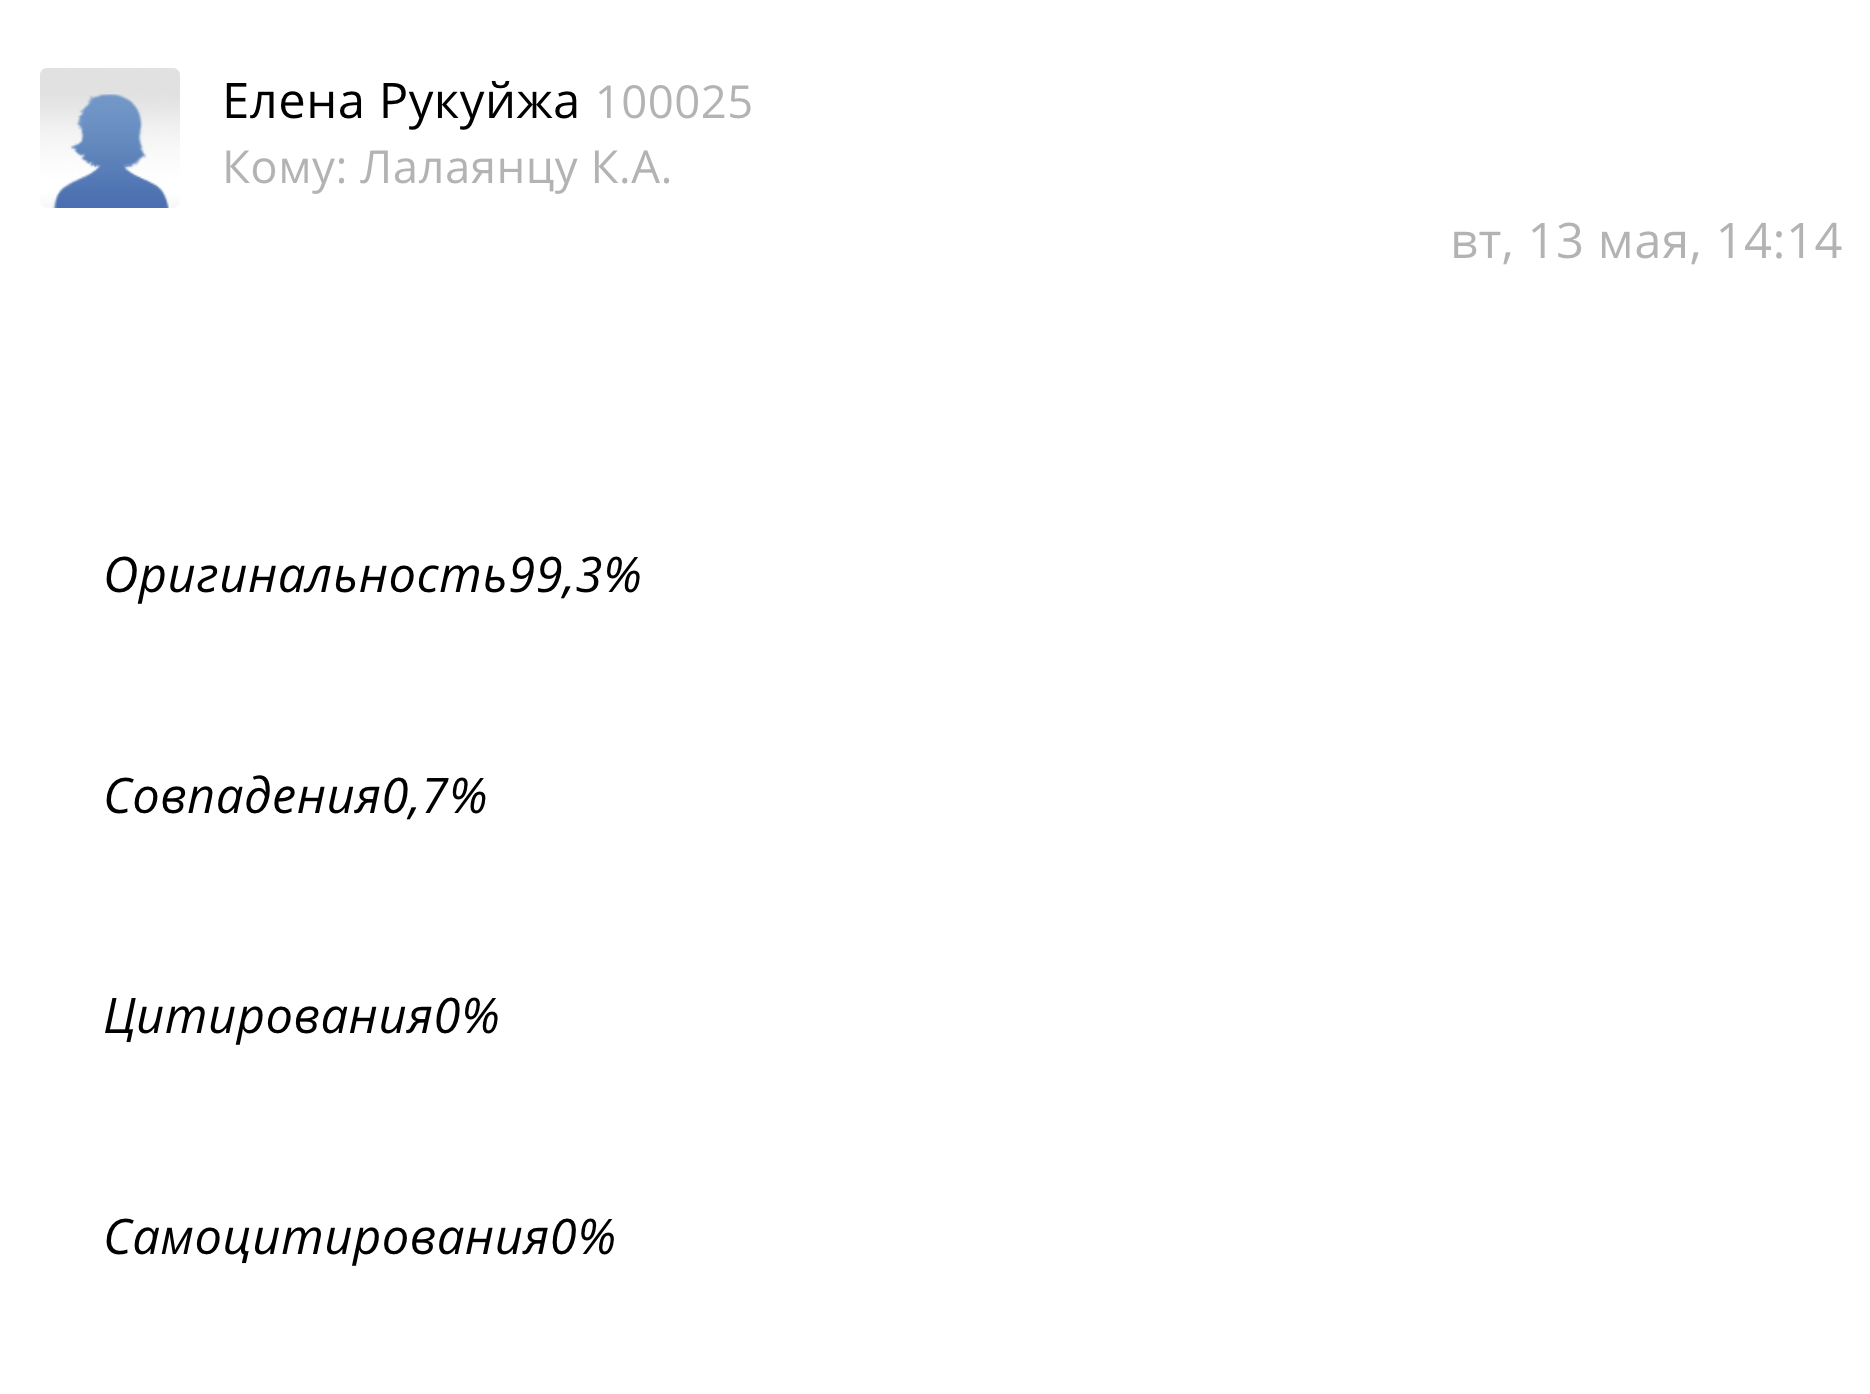
\includegraphics[width=0.8\linewidth]{images/presentation/antiplagiat.png}\\
  \small Результаты первой проверки на антиплагиат.
\end{frame}

\begin{frame}
  \frametitle{Информация для предзащиты}
  \framesubtitle{Модуль практики}
  \centering
  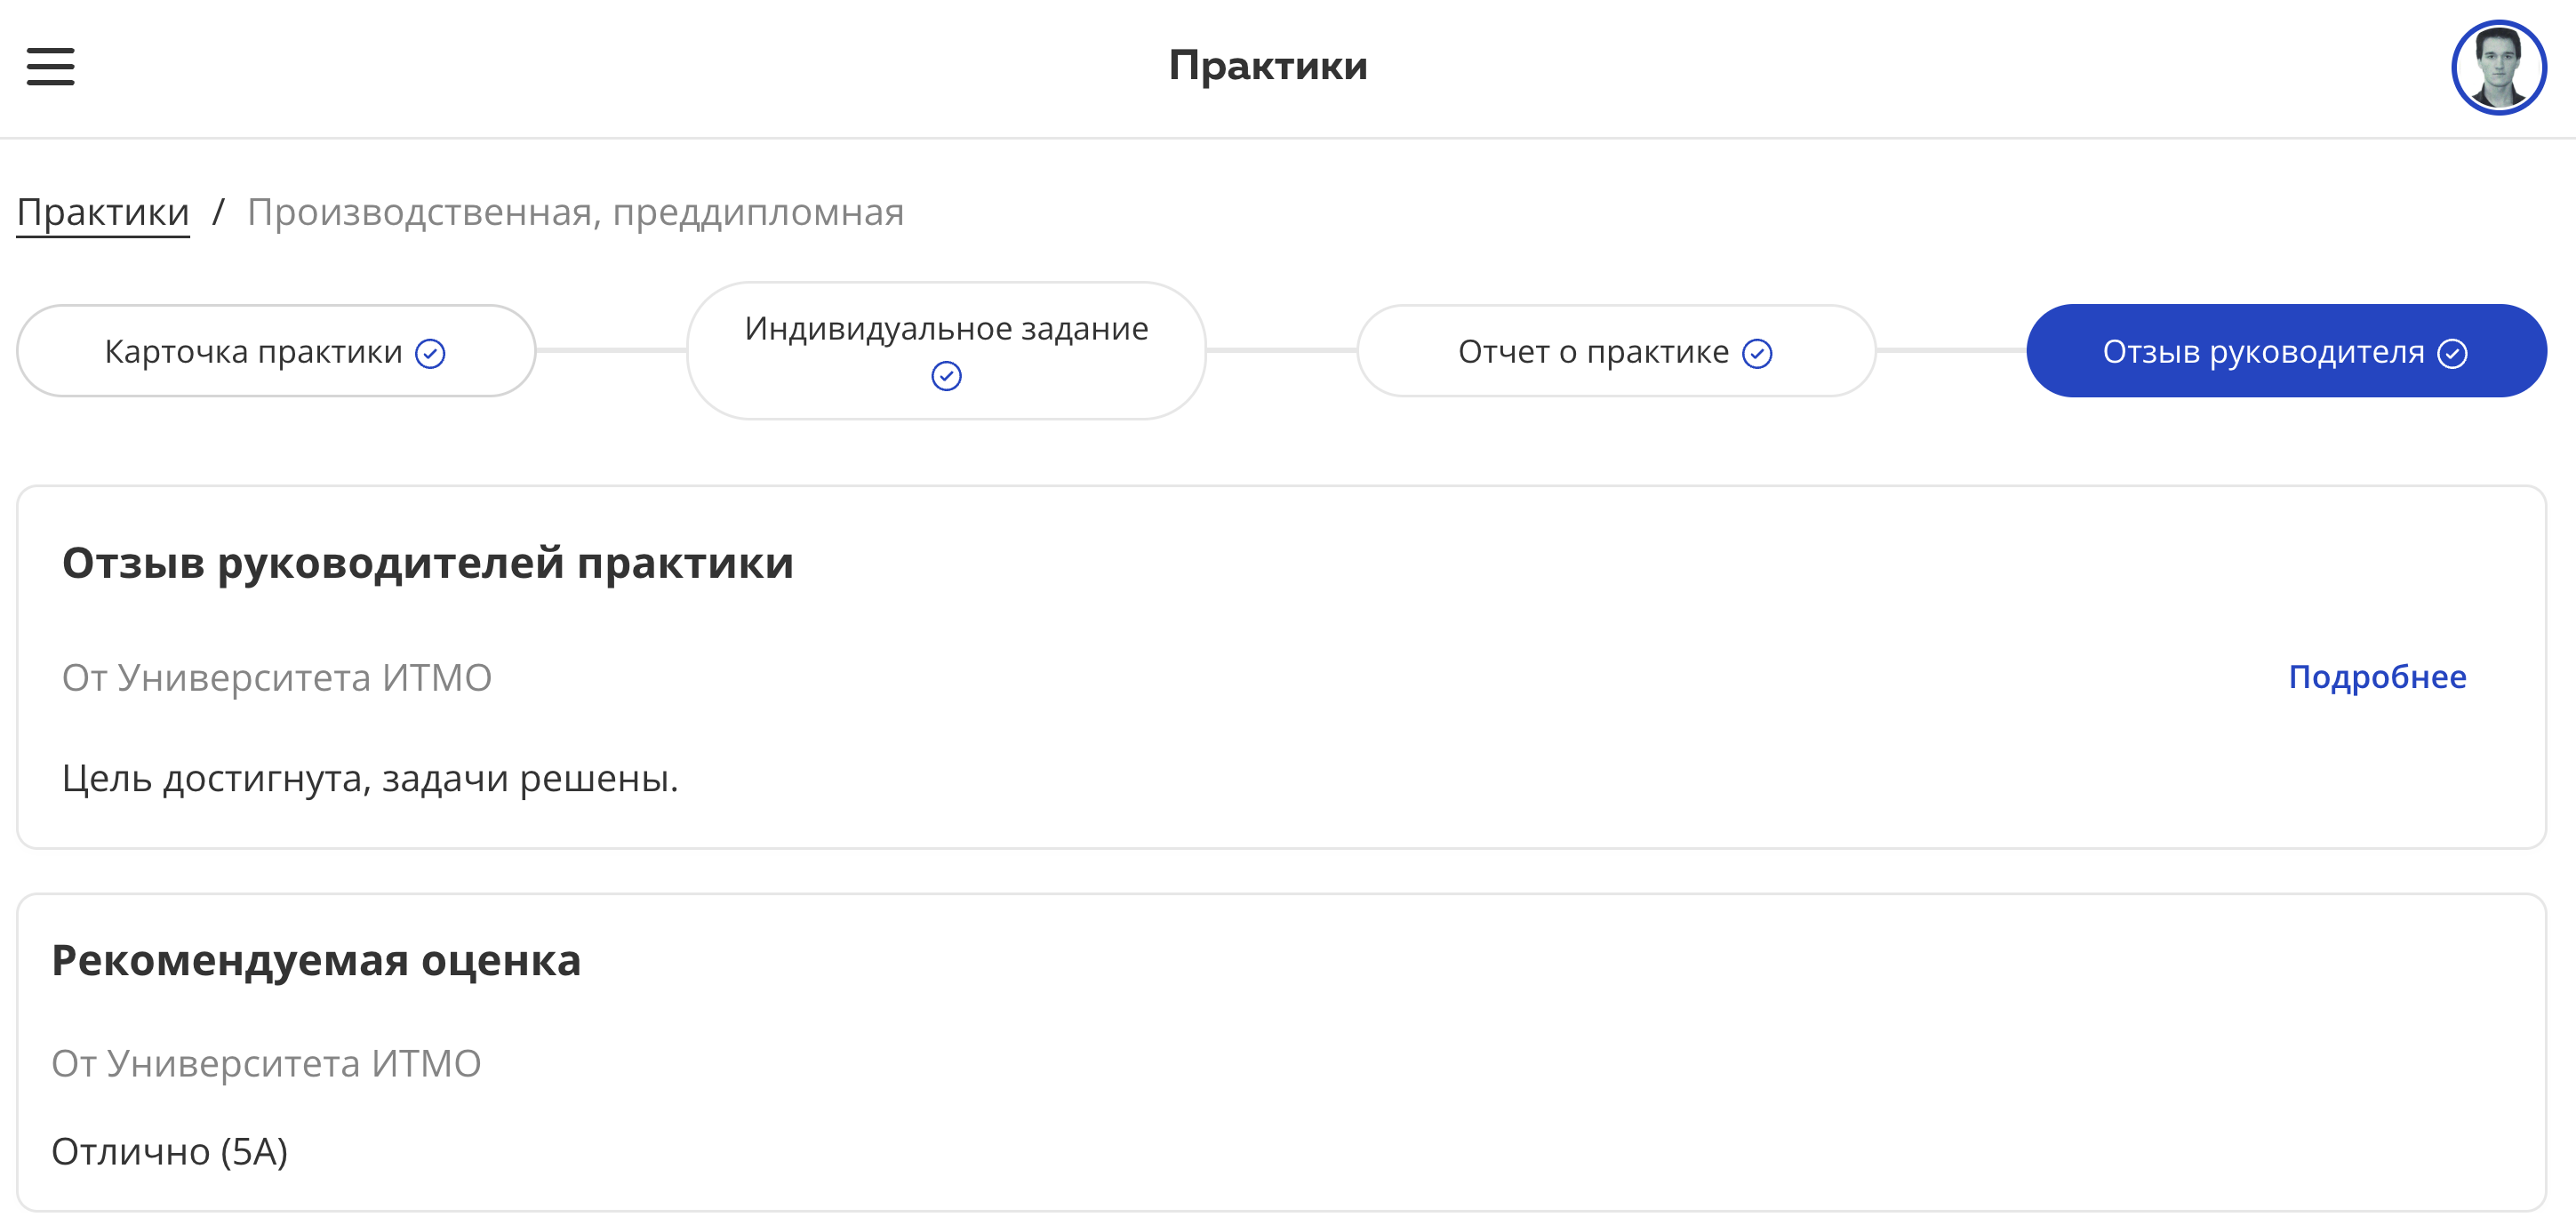
\includegraphics[width=1\linewidth]{images/presentation/practice.png}\\
  \small Оценка за практику.
\end{frame}

\begin{frame}{Задача отслеживания}
  \begin{itemize}
    \item Обработка видеоизображений для извлечения информации об объектах:
      \begin{itemize}
        \item детектирование объектов
        \item присвоение уникальных идентификаторов
        \item сохранение истории перемещений
      \end{itemize}
    \item Ключевые подходы:
      \begin{itemize}
        \item двухкомпонентные (ReID\footnote{ReID-модель (англ. Re-identification) -- нейронная сеть, задачей которой является исключительно создание векторов значений, позволяющих отличить объекты одного класса друг от друга.} + детектор) и однокомпонентные системы
        \item online и offline методы
        \item MOT\footnote{Отслеживание нескольких объектов (англ. Multiple Object Tracking)} и SOT\footnote{Отслеживание одного объекта (англ. Single Object Tracking)}
      \end{itemize}

  \end{itemize}
\end{frame}

% \begin{frame}{Актуальность}
%   \begin{columns}[T]
%     \begin{column}{\textwidth}
%       \textbf{Спортивная аналитика:}
%       \begin{itemize}
%         \item Отслеживание траектории мяча
%       \end{itemize}
%     \end{column}
%   \end{columns}
%   \vspace{0.5cm}
%   \begin{columns}
%     \begin{column}{0.5\textwidth}
%       \centering
%       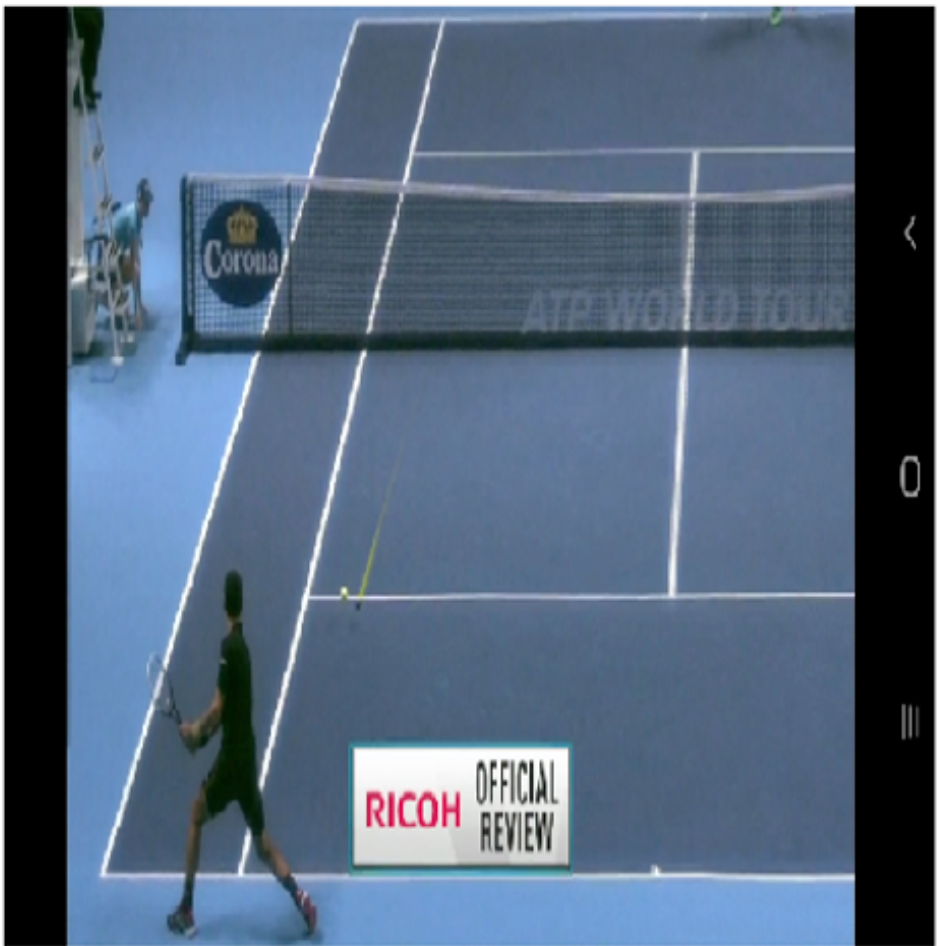
\includegraphics[width=\linewidth]{review/ball_track.png}
%       \small Спортивная аналитика
%     \end{column}
%   \end{columns}
% \end{frame}

\begin{frame}{Актуальность}
  \textbf{Урбанистика:}
  \begin{itemize}
    \item Подсчёт автомобилей и анализ движения на городских улицах
  \end{itemize}
  \vspace{0.5cm}
  \centering
  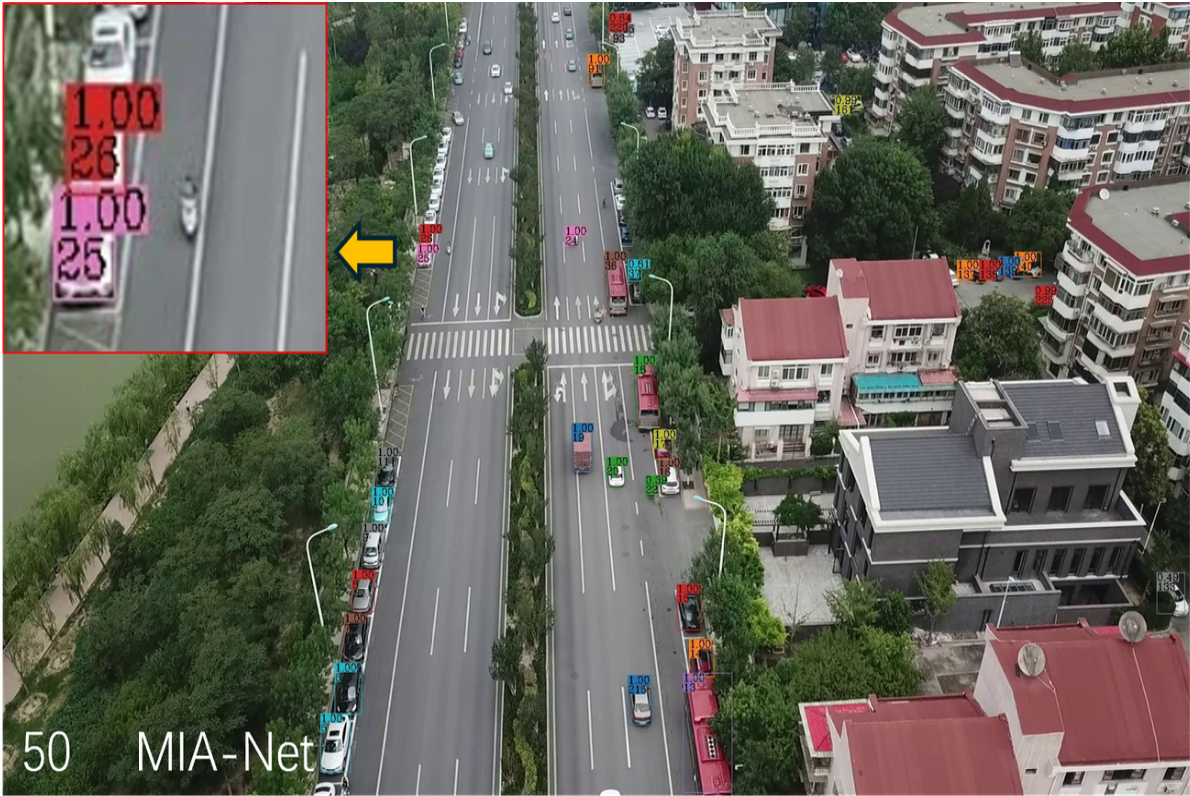
\includegraphics[width=0.7\linewidth]{review/urban_uav.png}\\
  \small Урбанистический анализ с использованием БПЛА
\end{frame}

\begin{frame}{Актуальность}
  \textbf{Робототехника:}
  \begin{itemize}
    % \item Обеспечение навигации и безопасности
    \item Следование за объектом
  \end{itemize}
  \vspace{0.5cm}
  \centering
  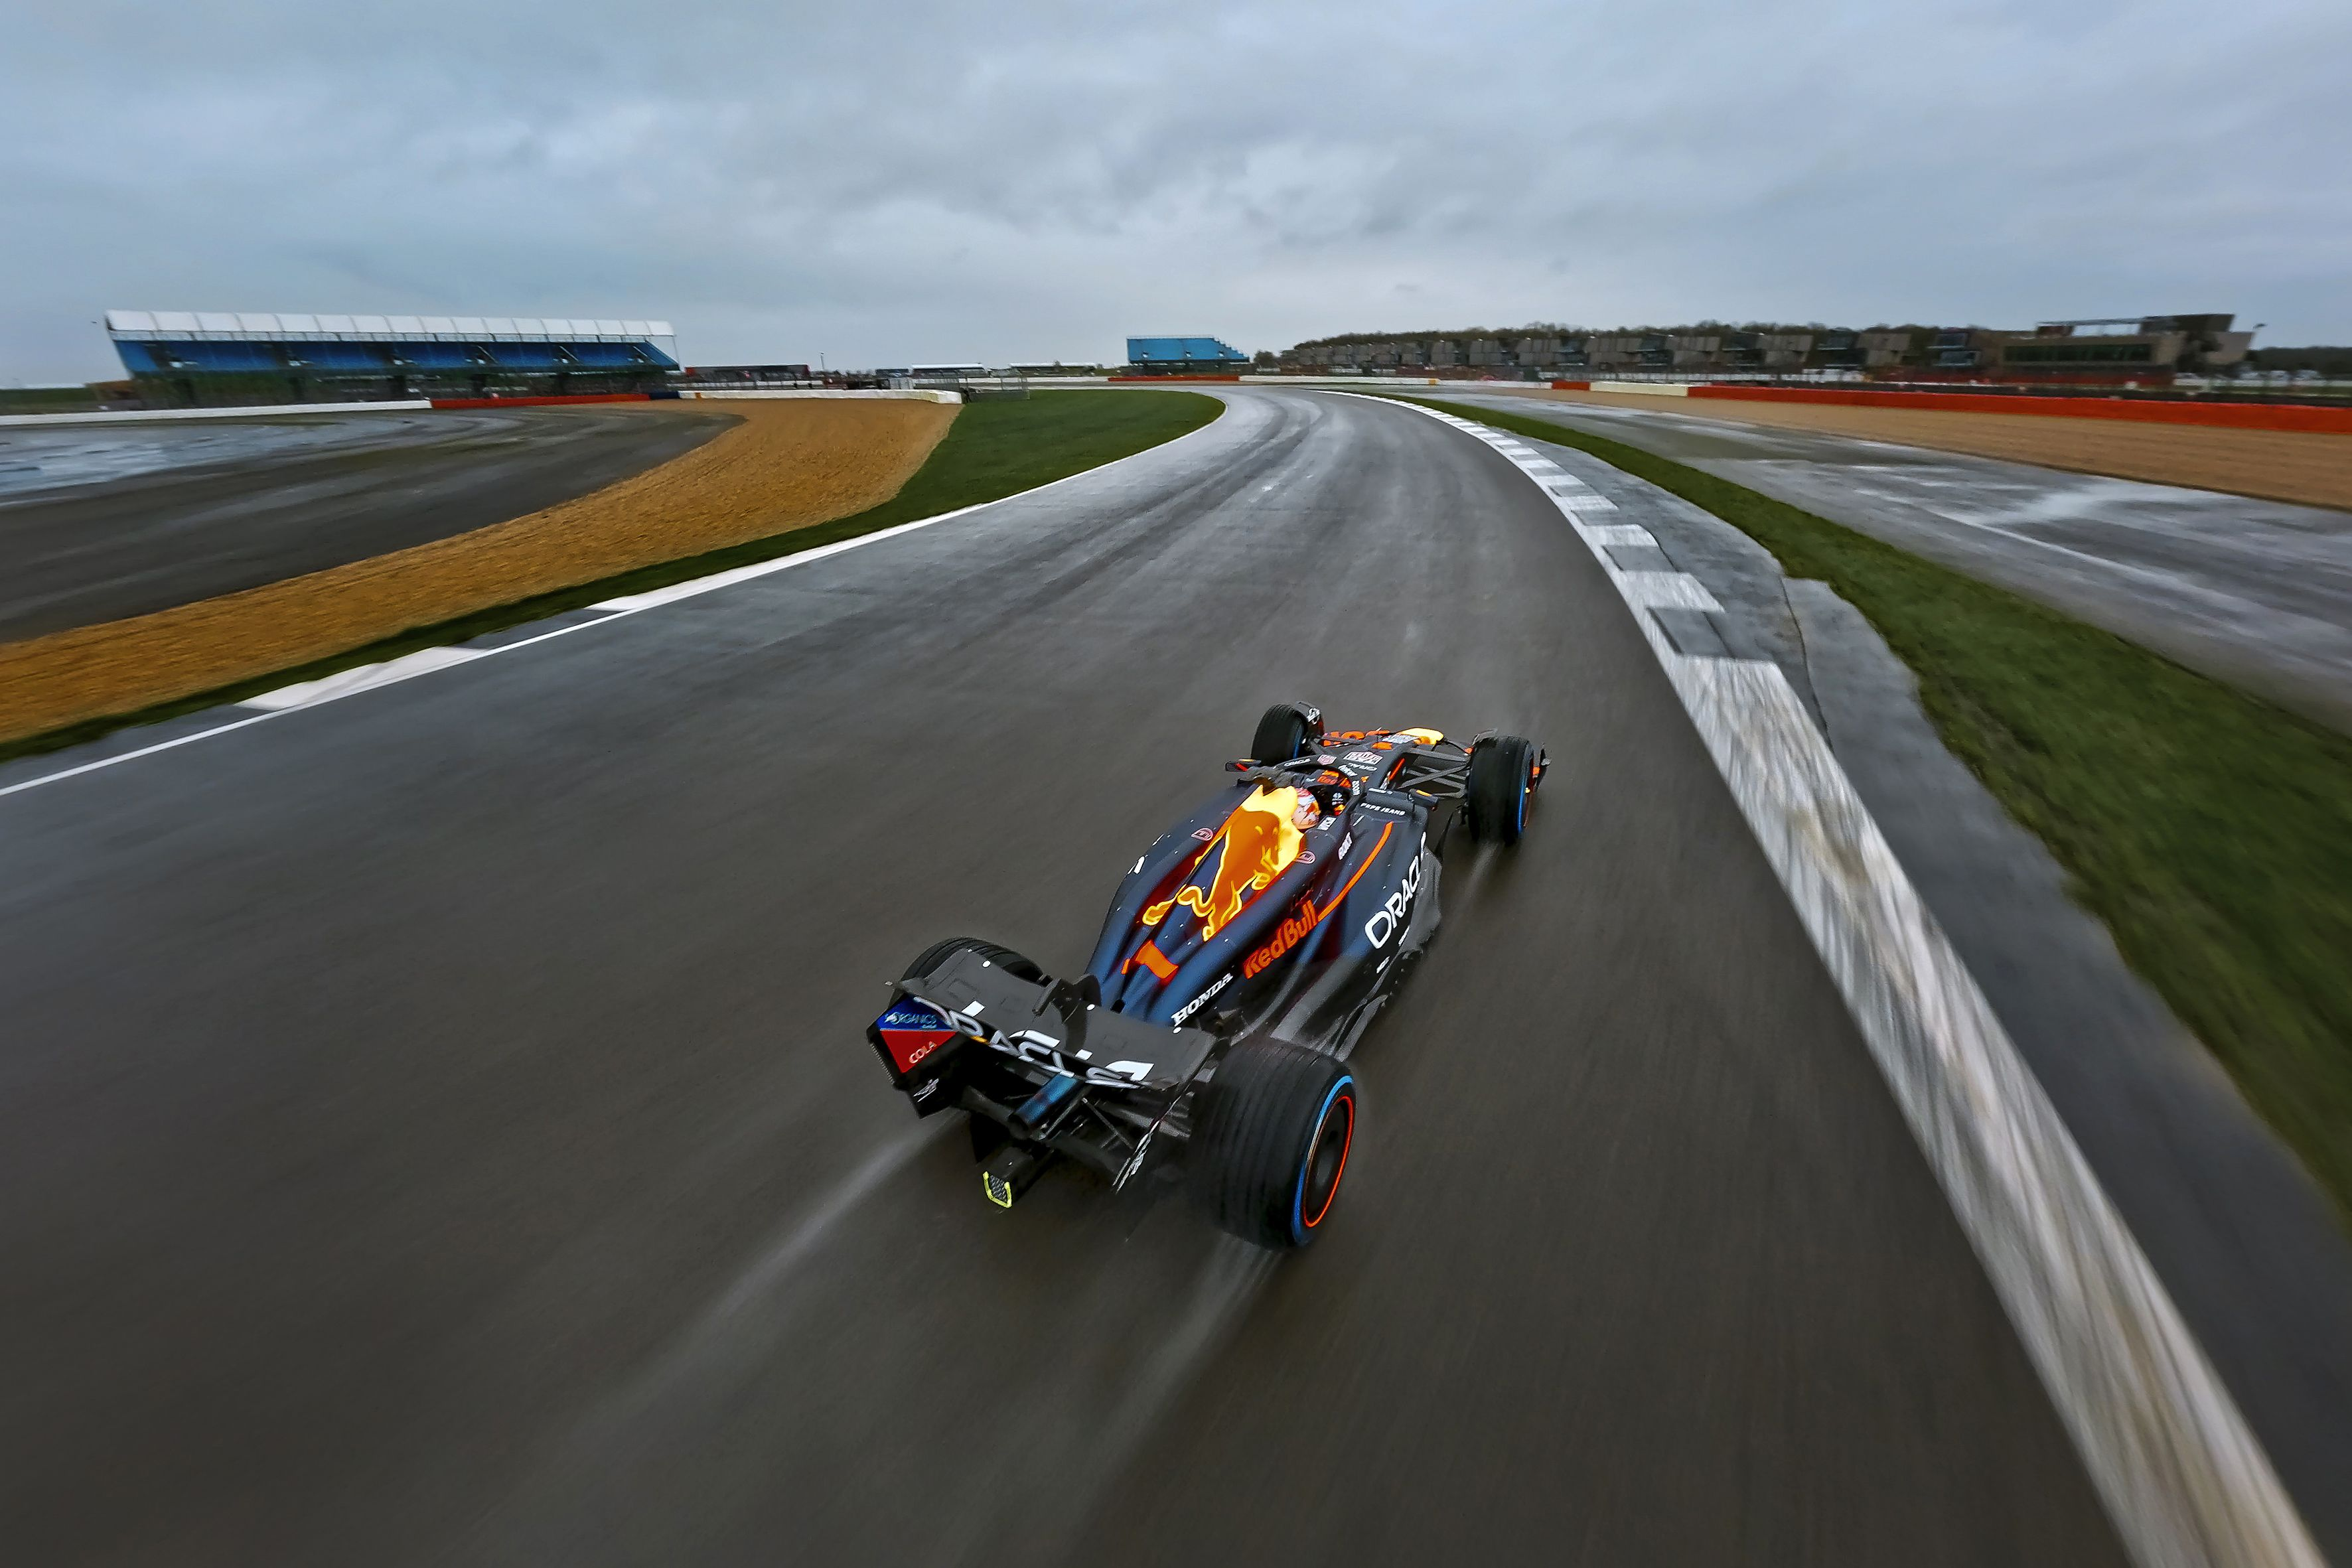
\includegraphics[width=0.7\linewidth]{presentation/f1_car.jpg}\\
  \small Кадр дрона оператора гонки F1
\end{frame}

\begin{frame}{Проблемы}
  \begin{columns}[T]
    \begin{column}{0.45\textwidth}
      \textbf{Проблемы:}
      \begin{itemize}
        \item Высокие требования к вычислительным ресурсам
        \item Задержки при централизованной обработки
        \item Риски потери данных и сбоев соединения
      \end{itemize}
    \end{column}
    \begin{column}{0.45\textwidth}
      \textbf{Решение:}
      \begin{itemize}
        \item Использование микрокомпьютера
        \item Локальная обработка данных в реальном времени
        \item Повышение автономности и отказоустойчивости системы
      \end{itemize}
    \end{column}
  \end{columns}
\end{frame}

\begin{frame}{Цель работы и практическая значимость}
  \begin{itemize}
    \item \textbf{Цель:} Выполнить сравнительный анализ существующих подходов к отслеживанию объектов в
    видеопотоке с целью выявления наиболее подходящих для низкопроизводительных
    устройств алгоритмов на основе показателей производительности и метрик.
    \item \textbf{Практическая значимость:}
      \begin{itemize}
        \item Разработка рекомендаций по выбору алгоритмов для работы в реальном времени.
        % \item Улучшение систем автономного управления и анализа данных.
      \end{itemize}
  \end{itemize}
\end{frame}

\begin{frame}{Задачи}
  Решаемые в ВКР задачи:
  \begin{enumerate}
    \item аналитический обзор существующих алгоритмов;
    \item подготовка стенда для апробации;
    \item подготовка экспериментов для сравнения различных алгоритмов на основании метрик HOTA, MOTA, IDF1 и показателей производительности;
    \item анализ полученных результатов и выработка рекомендации.
\end{enumerate}
\end{frame}

\begin{frame}
  \frametitle{Аналитический обзор}
  \framesubtitle{Датасет MOT17}
  \begin{itemize}
    \item 14 сцен с пешеходами в реальной городской среде.
    \item Сцены с разным углом съёмки, плотностью толпы, освещением.
    \item Есть аннотации координат и ID на каждый кадр.
    \item Применяется как стандарт для оценки трекеров.
  \end{itemize}
  \centering
  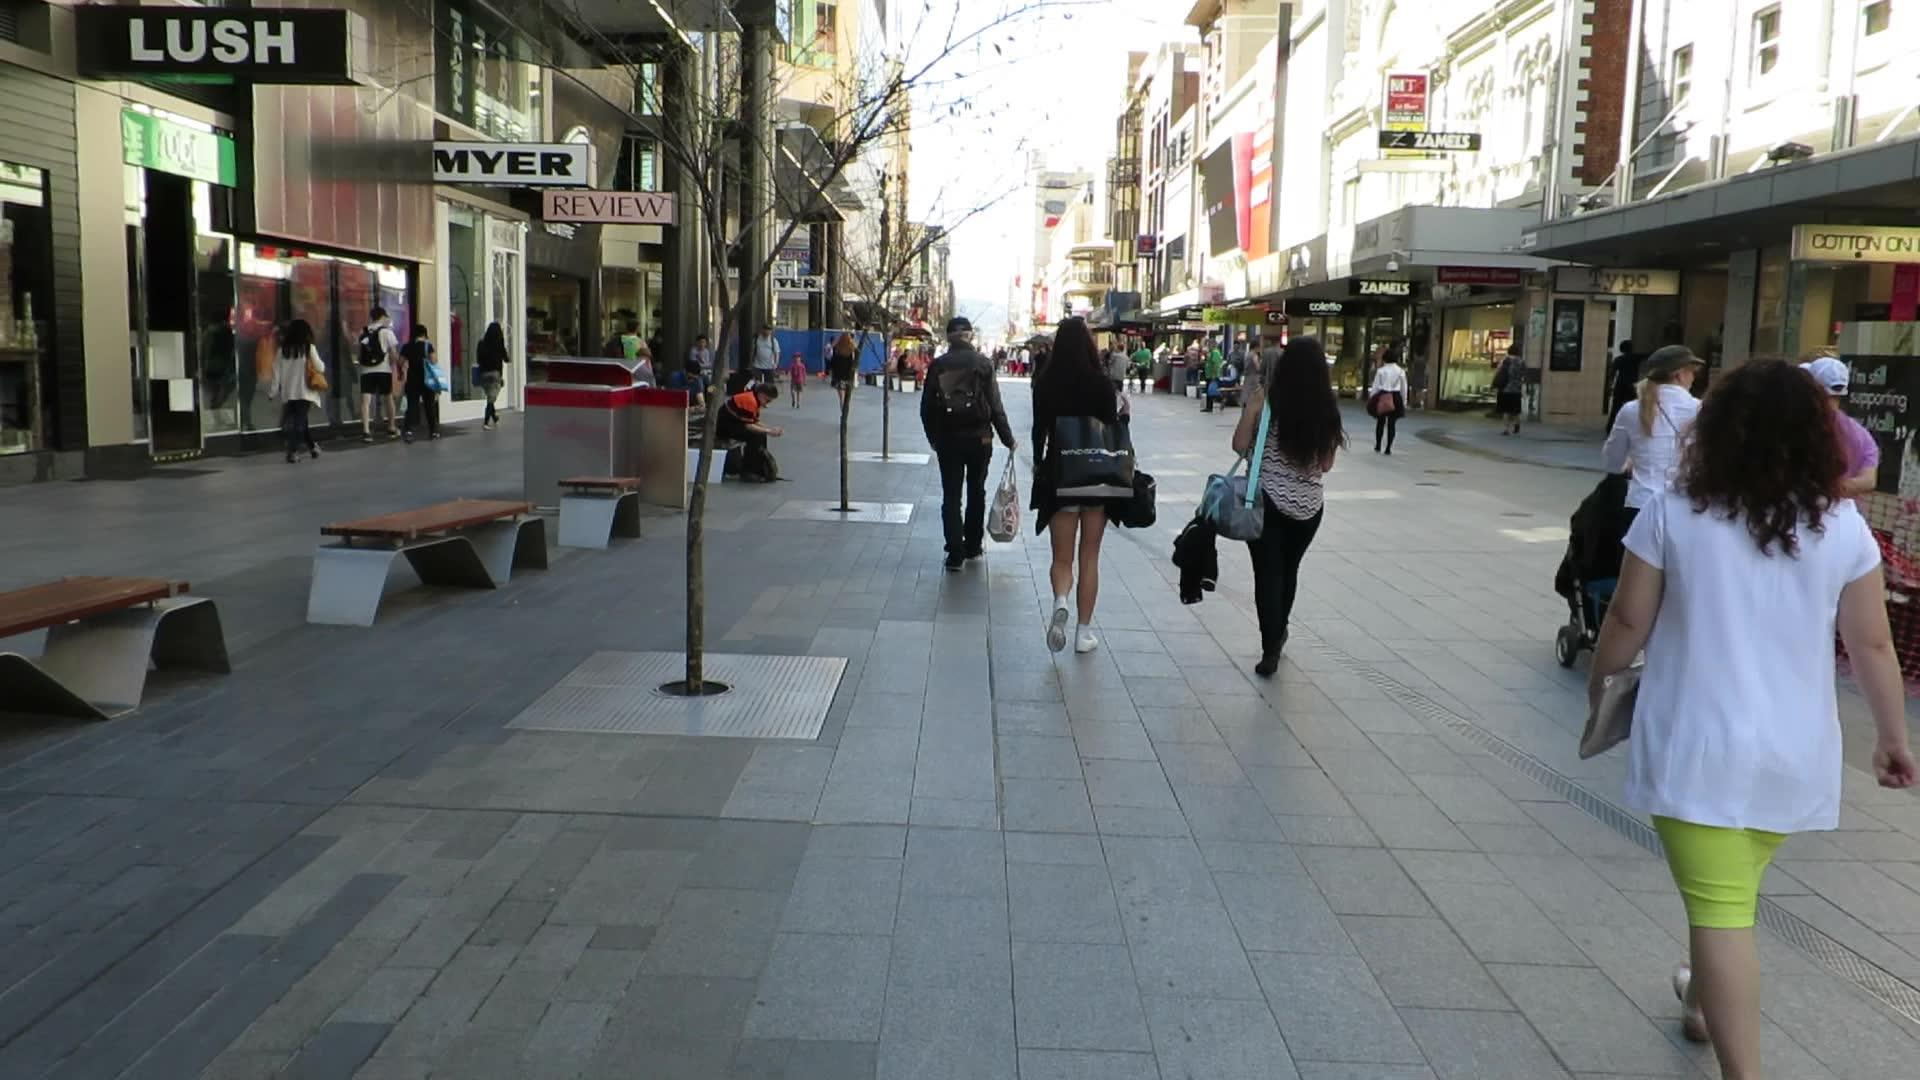
\includegraphics[width=0.7\linewidth]{images/review/MOT17_1.jpg}\\
  \small Пример изображения из MOT17.
\end{frame}

\begin{frame}
  \frametitle{Аналитический обзор}
  \framesubtitle{Метрики HOTA, MOTA, IDF1}
  \begin{itemize}
    \item \textbf{MOTA} — как хорошо найдены все объекты.
    \item \textbf{IDF1} — насколько трекер сохраняет ID.
    \item \textbf{HOTA} — баланс между нахождением и сохранением ID.
  \end{itemize}
  \centering
  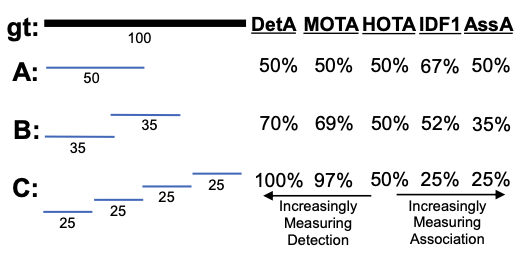
\includegraphics[width=0.7\linewidth]{images/presentation/metrics.png}\\
  \small Наглядный пример отличия метрик.
\end{frame}

\begin{frame}
  \frametitle{Аналитический обзор}
  \framesubtitle{Сравнение алгоритмов (1/2)}
  \begin{itemize}
    \item \textbf{ByteTrack:} ассоциация по IoU (сопоставление по максимизации совпадения площадей найденного объекта с известными), учитываются слабые детекции. Высокая полнота, но возможны ошибки идентичности.
    \item \textbf{OC-SORT:} меньшая чувствительность к шумам; откат и обновления состояния фильтра Калмана при кратковременной потери объекта, учёт нескольких прошлых наблюдений.
    \item \textbf{BoT-SORT:} IoU + ReID-модель, улучшенный вектор состояния фильтра Калмана.
  \end{itemize}
\end{frame}
\begin{frame}
  \frametitle{Аналитический обзор}
  \framesubtitle{Сравнение алгоритмов (2/2)}
  \begin{itemize}
    \item \textbf{StrongSORT:} компенсация движения камеры, улучшенное сопоставление траекторий, обновление визуальных особенностей экспоненциальным средним.
    \item \textbf{ImprAssOC:} единая ассоциация по всем детекциям, ReID + компенсация движения. Лучше сопоставляет при слабых детекциях.
    \item \textbf{Deep OC-SORT:} адаптивный коэффициент скользящего экспоненциального среднего (меньший учет новых особенностей при меньшей уверенности в детекции).
  \end{itemize}
\end{frame}

% \begin{frame}
%   \frametitle{Cтенд для апробации}
%   \framesubtitle{Выбор микрокомпьютера}
%   \begin{itemize}
%       \item \textbf{Nvidia Jetson} – высокая производительность, однако дорогой, тяжёлый и мало распространённый в РФ.
%       \item \textbf{Orange Pi} – аналог Raspberry Pi, но с худшей поддержкой и меньшей доступностью.
%       \item \textbf{Raspberry Pi} – оптимальный выбор: относительно недорогой, лёгкий (50 г), энергоэффективный, широко доступен.
%   \end{itemize}
% \end{frame}


% \begin{frame}
%   \frametitle{Cтенд для апробации}
%   \framesubtitle{Выбор вычислительного модуля}
%   \textbf{TPU} -- специализированный вычислительный модуль для параллельных вычислений тензоров.
%   \begin{itemize}
%       % \item \textbf{Hailo} – более новый и мощный, но требует переписывания кода;
%       \item \textbf{Google Coral} – проверенное решение: требует лишь конвертации весов модели в специальный формат; выпускается в различных форм-факторах (M.2, USB).
%   \end{itemize}
%   \centering
%   \includegraphics[width=0.5\linewidth]{images/presentation/tpu.png}\\
%   \small Google Coral на плате расширения.
% \end{frame}


\begin{frame}
  \frametitle{Cтенд для апробации}
  \framesubtitle{Аппаратная часть}
  \begin{itemize}
      \item По результатам анализа выбраны компоненты для экспериментального стенда:
      \begin{itemize}
          \item \textbf{Микрокомпьютер:} Raspberry Pi 5 (8 ГБ);
          \item \textbf{Вычислительный модуль:} Google Coral Dual TPU;
          \item \textbf{Плата расширения:} Pineboards AI Dual.
      \end{itemize}
      \item Цена комплекта ~28000 рублей, вес ~0.1 кг -- подходит для автономных устройств.
      
      \centering
  \includegraphics[width=0.5\linewidth]{images/presentation/tpu.png}\\
  \small Google Coral на плате расширения.
  \end{itemize}
\end{frame}

\begin{frame}
    \frametitle{Эксперименты}
    \framesubtitle{1. Влияние размера сети детектора на показатели качества}
    \begin{itemize}
      \item Большая модель YOLOv8 → выше HOTA, MOTA, IDF1.
      \item Увеличение разрешения изображения даёт больший прирост, чем размер модели.
      % \item Оптимум: YOLOv8n с разрешением 512 – хорошее качество при высокой скорости.
    \end{itemize}
    % Placeholder: график метрик vs размер сети и разрешение
    \centering
    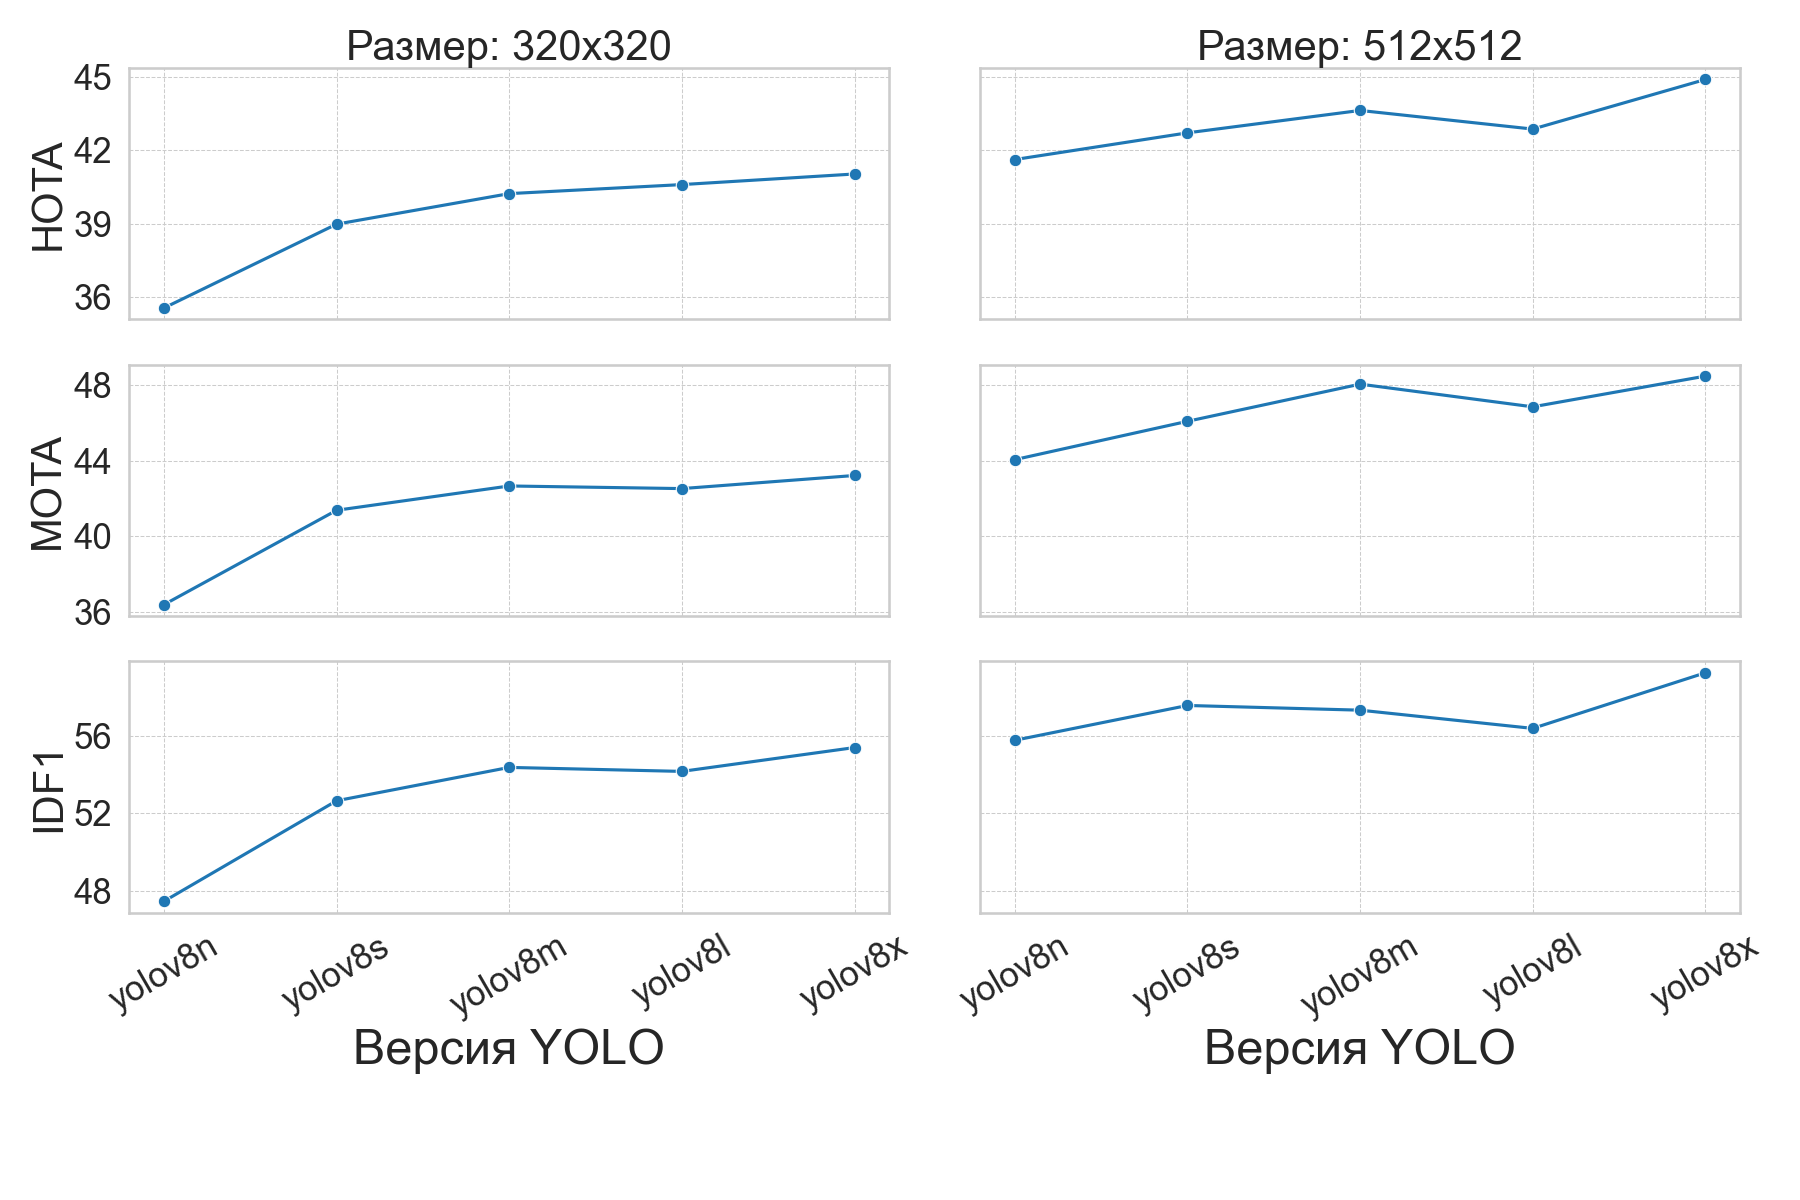
\includegraphics[width=0.7\linewidth]{images/plots/yolo_size_vs_metric/ByteTrack.png}\\
    \small Результаты эксперимента для алгоритма ByteTrack.
\end{frame}

\begin{frame}
  \frametitle{Эксперименты}
  \framesubtitle{2. Влияние ReID-модели на показатели качества}
  \begin{itemize}
    \item Значительного влияния ReID-модель не оказывает. Показатели качества незначительно колеблются.
  \end{itemize}
  % Placeholder: метрики IDF1, HOTA для разных ReID
  \centering
  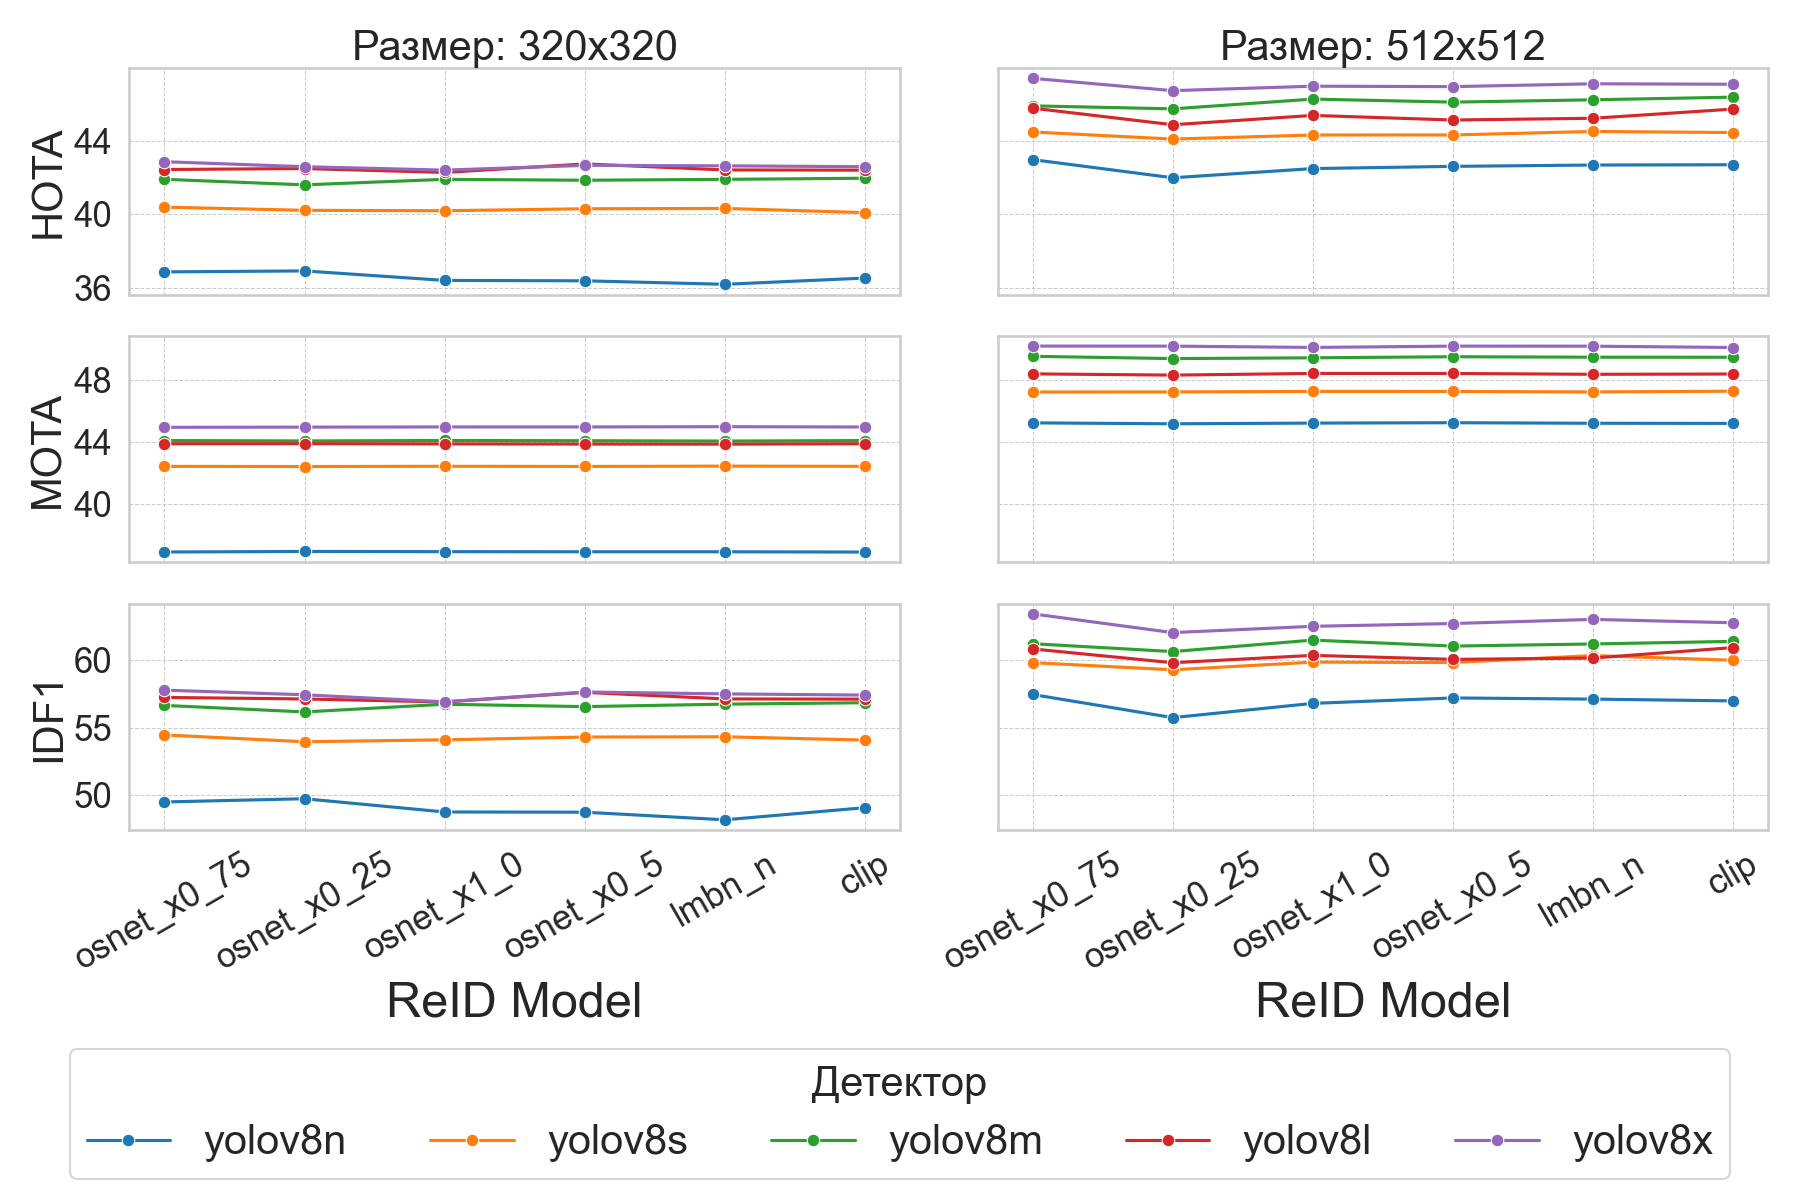
\includegraphics[width=0.7\linewidth]{images/plots/yolo_size_and_reid_vs_metric/BoT-SORT.png}\\
  \small Результаты эксперимента для алгоритма BoT-SORT.
\end{frame}

\begin{frame}
  \frametitle{Эксперименты}
  \framesubtitle{3. Влияние частоты кадров видеопотока на показатели качества}
  \begin{itemize}
    \item Метрики значительно улучшаются до 5 кадров/с
    \item 5-11 кадров/с — менее выраженный рост
    \item Выше 11 кадров/с нет значимого улучшения
  \end{itemize}
  % Placeholder: график HOTA, MOTA от FPS
  \centering
  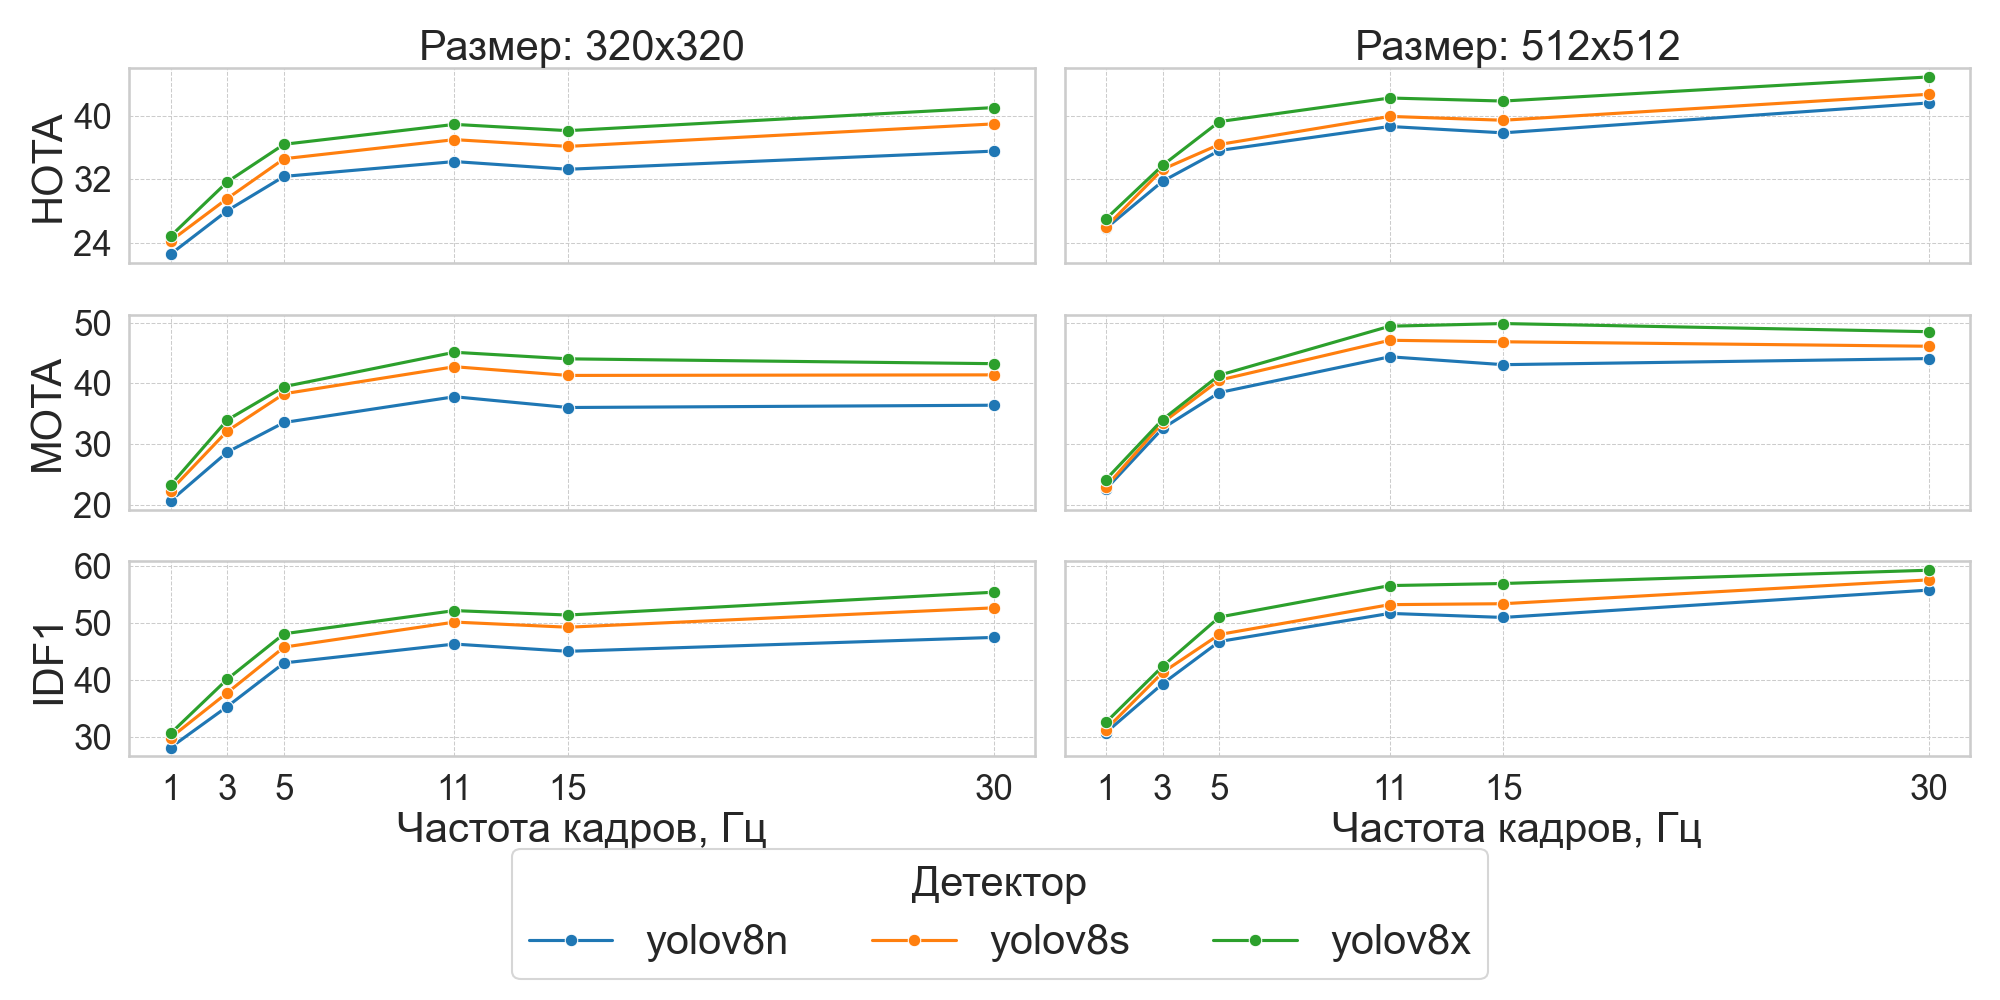
\includegraphics[width=0.7\linewidth]{images/plots/fps_vs_metric/ByteTrack.png}\\
  \small Результаты эксперимента для алгоритма ByteTrack.
\end{frame}

\begin{frame}
  \frametitle{Эксперименты}
  \framesubtitle{4. Влияние количества объектов в кадре на частоту работы}
  \begin{table}[htbp]
\caption{Корреляция частоты работы с количеством объектов на изображении}
\label{tab:correlation_fps_object}
\centering
\begin{tabular}{lr}
\toprule
Алгоритм & Корреляция \\
\midrule
BoT-SORT & -0.63 \\
ByteTrack & -0.03 \\
Deep OC-SORT & -0.65 \\
ImprAssOC & -0.63 \\
OC-SORT & -0.10 \\
StrongSORT & -0.66 \\
\bottomrule
\end{tabular}

\end{table}
  \begin{itemize}
    \item Алгоритмы ByteTrack, OC-SORT — демонстрируют почти нулевую корреляцию, лучший выбор при насыщенной объектами сцене.
    \item трекеры с ReID-моделями теряют FPS при росте числа целей.
  \end{itemize}

\end{frame}

\begin{frame}
  \frametitle{Эксперименты}
  \framesubtitle{Тепловые карты по результатам экспериментов}
  Две тепловые карты: с частотой работы и с метрикой HOTA для каждой пары алгоритма и ReID-модели. Чем ближе цвет ячейки к желтому -- тем лучше результат.

  \centering
  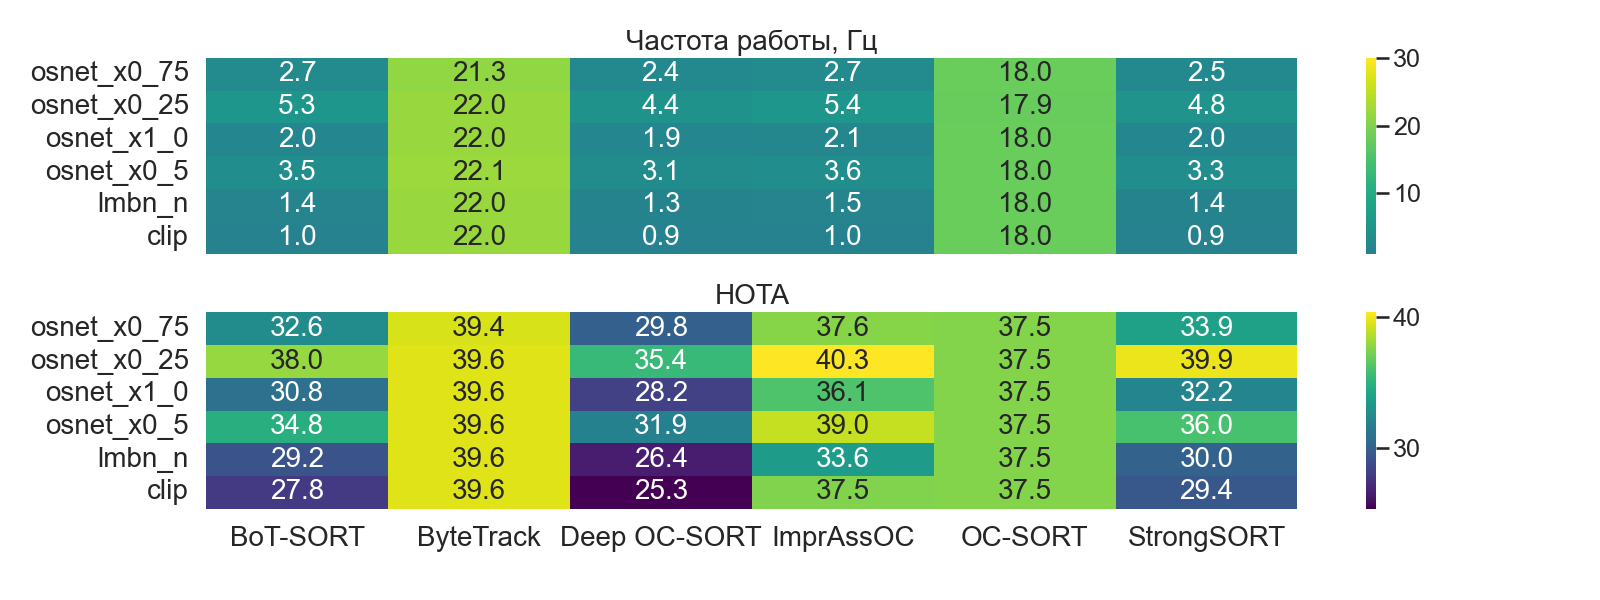
\includegraphics[width=\linewidth]{images/plots/heatmap_fps_hota_vs_tracker_reid/heatmap_fps_hota_yolov8n_size512.png}\\
  \small Тепловая карта для YOLOv8n на размере изображения 512.
\end{frame}


\begin{frame}
  \frametitle{Анализ полученных результатов}
  \framesubtitle{Выводы по результатам экспериментов}
  \begin{itemize}
    % \item Использование RP5 c TPU позволяет запустить современные алгоритмы.
    \item YOLOv8n выигрывает благодаря скорости работы.
    \item Алгоритм ByteTrack наиболее стабильный результат благодаря высокой частоте работы, имеет потенциал для увеличения качества изображения. Подходит для сцен с большой плотностью объектов, например, подсчета пешеходов на улице.
    \item Алгоритмы ImprAssOC и StrongSORT показывают высокие показатели качества при использовании в паре с OSNet X0.25 на изображении размера 512. Могут быть использованы при медленном движении малого (не более 5) количества объектов, например, очередь в магазине.
    \item Алгоритмы OC-Sort, BoT-SORT и DeepOC-SORT не рекомендуются к использованию.
  \end{itemize}
\end{frame}

\begin{frame}{Заключение}
  \begin{itemize}
    \item Изучены современные алгоритмы трекинга и их применимость на маломощных устройствах.
    \item Собран экспериментальный стенд на Raspberry Pi 5 с TPU.
    \item Проведены тесты на MOT17: сравнение 6 алгоритмов по метрикам качества и скорости.
    \item Проведен анализ полученных результатов.
    \item Задачи выполнены, цель достигнута — выявлены решения подходящие для работы в реальном времени на низкопроизводительных устройствах.
  \end{itemize}
\end{frame}


\begin{frame}
  \centering \Huge \textcolor{blue}{Спасибо за внимание!}
\end{frame}

\end{document}
